% ============================================================
% Recueil COMIMa — Techniques de résolution de problèmes
% Chapitre 8 — Inégalités
% D'après A. Engel, Problem-Solving Strategies (Springer, 1998), chap. 7.
%
% Compilation (paquet .tex exporté) : latexmk -pdf cours.tex
% Les énoncés et solutions des exercices sont inclus depuis
% <id>/enonce.tex et <id>/solution.tex (content/exercices/ sur le dépôt).
% ============================================================
\documentclass[11pt]{article}
\input{preamble.tex}
\input{preamble-cours.tex}

% Solutions en fin de chapitre : \solutionsfalse pour les masquer.
\solutionstrue

\begin{document}

\chapitre{8}{Inégalités}

Comparer deux quantités sans pouvoir les calculer : c'est l'objet des
inégalités, omniprésentes dans les compétitions. Quelques outils suffisent
à en traiter un très grand nombre : la positivité des carrés, les
inégalités entre moyennes, l'inégalité de Cauchy--Schwarz et l'inégalité
de réordonnement. Dans les problèmes de géométrie, l'inégalité triangulaire
joue en plus un rôle central.

\medskip
{\small\itshape Ce chapitre suit le chapitre 7 de A.~Engel,
\emph{Problem-Solving Strategies}, Springer, 1998.}

% ------------------------------------------------------------
\section{Le point de départ : un carré est positif}\label{sec:point-de-depart}

Pour tout réel $x$ et tous réels $x_1, \ldots, x_n$,
\[
x^2 \geqslant 0, \qquad \sum_{i=1}^{n} x_i^2 \geqslant 0,
\]
avec égalité si et seulement si $x = 0$, respectivement
$x_1 = \cdots = x_n = 0$.

Une stratégie générale consiste à transformer l'inégalité à démontrer en
une inégalité équivalente de cette forme. Le chemin est souvent long ; on
établit donc une fois pour toutes quelques conséquences utiles.

\begin{exemple}\label{exm:E5}
Pour tous réels $a$, $b$, $c$,
\[
a^2 + b^2 + c^2 \geqslant ab + bc + ca,
\]
avec égalité si et seulement si $a = b = c$.
\end{exemple}

\begin{proof}
En multipliant par $2$, l'inégalité équivaut à
\[
2a^2 + 2b^2 + 2c^2 - 2ab - 2bc - 2ca \geqslant 0
\iff (a-b)^2 + (b-c)^2 + (c-a)^2 \geqslant 0,
\]
qui est vraie. L'égalité a lieu si et seulement si $a - b = b - c = c - a = 0$, c'est-à-dire
$a = b = c$.
\end{proof}

% ------------------------------------------------------------
\section{Moyennes de deux nombres}\label{sec:moyennes-deux-nombres}

\begin{definition}
Soient $a, b > 0$. On appelle respectivement moyenne \emph{harmonique},
\emph{géométrique}, \emph{arithmétique} et \emph{quadratique} de $a$ et $b$
les nombres
\[
H = \frac{2ab}{a+b}, \qquad G = \sqrt{ab}, \qquad A = \frac{a+b}{2},
\qquad Q = \sqrt{\frac{a^2+b^2}{2}} .
\]
\end{definition}

\begin{theoreme}[Moyennes de deux nombres]\label{thm:moy2}
Pour tous $a, b > 0$,
\[
\min(a, b) \leqslant \frac{2ab}{a+b} \leqslant \sqrt{ab} \leqslant \frac{a+b}{2}
\leqslant \sqrt{\frac{a^2+b^2}{2}} \leqslant \max(a, b).
\]
Chacune de ces inégalités est une égalité si et seulement si $a = b$.
\end{theoreme}

\begin{proof}
Toutes les quantités sont strictement positives, ce qui permet d'élever au
carré, d'extraire des racines et de multiplier par des nombres positifs sans
changer le sens des inégalités.
\begin{itemize}
  \item $A \leqslant Q$ : $\left(\frac{a+b}{2}\right)^2 \leqslant \frac{a^2+b^2}{2}
  \iff (a+b)^2 \leqslant 2(a^2 + b^2) \iff 0 \leqslant (a-b)^2$.
  \item $G \leqslant A$ : $2\sqrt{ab} \leqslant a + b \iff
  0 \leqslant \left(\sqrt a - \sqrt b\right)^2$.
  \item $H \leqslant G$ : en multipliant par $\frac{a+b}{\sqrt{ab}} > 0$,
  $\frac{2ab}{a+b} \leqslant \sqrt{ab} \iff 2\sqrt{ab} \leqslant a + b$,
  ce qui est l'inégalité précédente.
  \item Les inégalités extrêmes : supposons $a \leqslant b$ (les rôles sont
  symétriques). Alors $\frac{2ab}{a+b} \geqslant a \iff 2b \geqslant a + b
  \iff b \geqslant a$, et $\frac{a^2 + b^2}{2} \leqslant b^2 \iff a^2 \leqslant b^2$.
\end{itemize}
Dans chaque cas, l'égalité équivaut à $a = b$.
\end{proof}

\begin{remarque}
L'inégalité $a^2 + b^2 \geqslant 2ab$ admet plusieurs formes équivalentes
qu'il faut savoir reconnaître : pour $a, b > 0$,
\[
\frac ab + \frac ba \geqslant 2, \qquad\text{et, pour } x > 0,\qquad
x + \frac1x \geqslant 2 ,
\]
avec égalité si et seulement si $a = b$, respectivement $x = 1$. Plus
généralement, pour $c > 0$ et $x > 0$, l'inégalité $G \leqslant A$
appliquée à $x$ et $\frac cx$ donne
\[
x + \frac cx \geqslant 2\sqrt c ,
\]
avec égalité si et seulement si $x = \frac cx$, c'est-à-dire $x = \sqrt c$.
\end{remarque}

\begin{exemple}\label{exm:E2}
Pour tous $a, b, c \geqslant 0$,
\[
(a+b)(b+c)(c+a) \geqslant 8abc .
\]
\end{exemple}

\begin{proof}
L'inégalité $\frac{x+y}{2} \geqslant \sqrt{xy}$ reste vraie pour
$x, y \geqslant 0$ (elle équivaut à $(\sqrt x - \sqrt y)^2 \geqslant 0$). En
multipliant les trois inégalités entre nombres positifs
\[
\frac{a+b}{2} \geqslant \sqrt{ab}, \qquad
\frac{b+c}{2} \geqslant \sqrt{bc}, \qquad
\frac{c+a}{2} \geqslant \sqrt{ca},
\]
on obtient $\frac{(a+b)(b+c)(c+a)}{8} \geqslant \sqrt{a^2b^2c^2} = abc$.

\emph{Cas d'égalité.} Si $abc > 0$, les trois inégalités portent sur des
nombres strictement positifs, et le produit est une égalité si et seulement
si chacune l'est : $a = b = c$. Si $abc = 0$, par exemple $a = 0$, le membre
de gauche vaut $bc(b + c)$, nul si et seulement si $b = 0$ ou $c = 0$.
L'égalité a donc lieu si et seulement si $a = b = c$ ou si deux des nombres
sont nuls.
\end{proof}

\begin{exemple}\label{exm:E3}
Si $a_1, \ldots, a_n > 0$ et $a_1 a_2 \cdots a_n = 1$, alors
\[
(1 + a_1)(1 + a_2) \cdots (1 + a_n) \geqslant 2^n .
\]
\end{exemple}

\begin{proof}
Pour chaque $i$, $\frac{1 + a_i}{2} \geqslant \sqrt{1 \cdot a_i} = \sqrt{a_i}$.
En multipliant ces $n$ inégalités entre nombres strictement positifs :
\[
\frac{1 + a_1}{2} \cdot \frac{1 + a_2}{2} \cdots \frac{1 + a_n}{2}
\geqslant \sqrt{a_1 a_2 \cdots a_n} = 1 .
\]
Il y a égalité si et seulement si $a_1 = \cdots = a_n = 1$.
\end{proof}

% ------------------------------------------------------------
\section{Le cas général : moyennes de \texorpdfstring{$n$}{n} nombres}\label{sec:moyennes-n-nombres}

\begin{definition}
Soient $x_1, \ldots, x_n > 0$. On définit
\begin{gather*}
H = \frac{n}{\frac{1}{x_1} + \cdots + \frac{1}{x_n}}, \qquad
G = \sqrt[n]{x_1 \cdots x_n}, \\
A = \frac{x_1 + \cdots + x_n}{n}, \qquad
Q = \sqrt{\frac{x_1^2 + \cdots + x_n^2}{n}} .
\end{gather*}
\end{definition}

\begin{theoreme}[Inégalités des moyennes]\label{thm:moyn}
Pour tous $x_1, \ldots, x_n > 0$,
\[
\min_i x_i \leqslant H \leqslant G \leqslant A \leqslant Q \leqslant \max_i x_i .
\]
Chacune de ces inégalités est une égalité si et seulement si
$x_1 = x_2 = \cdots = x_n$.
\end{theoreme}

Ce théorème est à connaître parfaitement : en compétition, on l'applique
sans le redémontrer. L'inégalité $G \leqslant A$ est appelée
\emph{inégalité arithmético-géométrique} (IAG). La démonstration est
répartie dans la suite du chapitre :
\begin{itemize}
  \item $\min_i x_i \leqslant H$ : si $m = \min_i x_i$, alors
  $\frac{1}{x_i} \leqslant \frac1m$ pour tout $i$, donc
  $\sum_i \frac1{x_i} \leqslant \frac nm$, soit $H \geqslant m$ ; de même
  $Q \leqslant \max_i x_i$. Égalité si et seulement si tous les $x_i$ sont égaux ;
  \item $A \leqslant Q$ : proposition~\ref{cor:QM} (Cauchy--Schwarz) ;
  \item $G \leqslant A$ : théorème~\ref{thm:IAG} (réordonnement) ;
  \item $H \leqslant G$ : proposition~\ref{cor:HG}.
\end{itemize}

% ------------------------------------------------------------
\section{L'inégalité de Cauchy--Schwarz}\label{sec:cauchy-schwarz}

\begin{theoreme}[Cauchy--Schwarz]\label{thm:CS}
Soient $a_1, \ldots, a_n$ et $b_1, \ldots, b_n$ des réels. Alors
\[
\Bigl(\sum_{i=1}^{n} a_i b_i\Bigr)^2 \leqslant \Bigl(\sum_{i=1}^{n} a_i^2\Bigr)\Bigl(\sum_{i=1}^{n} b_i^2\Bigr),
\]
avec égalité si et seulement si les vecteurs $\vec a = (a_1, \ldots, a_n)$
et $\vec b = (b_1, \ldots, b_n)$ sont colinéaires.
\end{theoreme}

\begin{proof}
Si tous les $a_i$ sont nuls, les deux membres sont nuls et $\vec a = \vec 0$
est colinéaire à $\vec b$. Sinon, posons $\alpha = \sum a_i^2 > 0$,
$\beta = \sum a_i b_i$, $\gamma = \sum b_i^2$. Pour tout réel $t$,
\[
P(t) = \sum_{i=1}^{n} (a_i t + b_i)^2 = \alpha t^2 + 2\beta t + \gamma \geqslant 0 .
\]
Le trinôme $P$, de coefficient dominant $\alpha > 0$, ne prend que des
valeurs positives : son discriminant est négatif ou nul,
$4\beta^2 - 4\alpha\gamma \leqslant 0$, c'est l'inégalité annoncée.

Si $\beta^2 = \alpha\gamma$, alors $t_0 = -\beta/\alpha$ est racine de $P$ ;
une somme de carrés nulle a tous ses termes nuls, donc $b_i = -t_0 a_i$ pour
tout $i$ : les vecteurs sont colinéaires. Réciproquement, si
$\vec b = \lambda \vec a$, les deux membres valent $\lambda^2 \alpha^2$.
\end{proof}

Avec le produit scalaire, l'inégalité s'écrit
$\left(\vec a \cdot \vec b\right)^2 \leqslant \|\vec a\|^2\,\|\vec b\|^2$.

\begin{proposition}\label{cor:QM}
Pour tous $x_1, \ldots, x_n > 0$, $A \leqslant Q$, avec égalité si et seulement
si tous les $x_i$ sont égaux.
\end{proposition}

\begin{proof}
Le théorème~\ref{thm:CS} appliqué à $(1, \ldots, 1)$ et $(x_1, \ldots, x_n)$
donne $(x_1 + \cdots + x_n)^2 \leqslant n\,(x_1^2 + \cdots + x_n^2)$. En
divisant par $n^2$ et en prenant la racine carrée (les deux membres sont
positifs), on obtient $A \leqslant Q$. L'égalité équivaut à la colinéarité
de $(x_1, \ldots, x_n)$ avec $(1, \ldots, 1)$, c'est-à-dire à
$x_1 = x_2 = \cdots = x_n$.
\end{proof}

\begin{exemple}
Soient $a, b > 0$. Pour $x \in \left]0, \frac\pi2\right[$,
\[
(a \sin x + b \cos x)^2 \leqslant (a^2 + b^2)(\sin^2 x + \cos^2 x) = a^2 + b^2 .
\]
Donc $a\sin x + b\cos x \leqslant \sqrt{a^2 + b^2}$, avec égalité si et
seulement si $(\sin x, \cos x)$ est colinéaire à $(a, b)$, c'est-à-dire
si $\tan x = \frac ab$. Cette valeur de $x$ existe dans $\left]0, \frac\pi2\right[$ :
le maximum de $a\sin x + b\cos x$ vaut exactement $\sqrt{a^2 + b^2}$.
\end{exemple}

% ------------------------------------------------------------
\section{L'inégalité de réordonnement}\label{sec:reordonnement}

Quatre boîtes contiennent des billets de $10$, $20$, $50$ et $100$ ariary ;
on peut prendre $3$, $4$, $5$ et $6$ billets, en choisissant librement à
quelle boîte s'applique chaque nombre. Pour gagner le plus, on prend le plus
de billets possible dans la boîte la plus riche : $6$ billets de $100$, puis
$5$ de $50$, $4$ de $20$ et $3$ de $10$. Pour gagner le moins, on fait
l'inverse. Le théorème suivant justifie cette intuition.

\begin{theoreme}[Inégalité de réordonnement]\label{thm:reord}
Soient $a_1 \leqslant a_2 \leqslant \cdots \leqslant a_n$ et
$b_1 \leqslant b_2 \leqslant \cdots \leqslant b_n$ des réels, et $\sigma$ une
permutation de $\{1, \ldots, n\}$. Alors
\[
\sum_{i=1}^{n} a_i b_{n+1-i} \;\leqslant\; \sum_{i=1}^{n} a_i b_{\sigma(i)}
\;\leqslant\; \sum_{i=1}^{n} a_i b_i .
\]
La somme est maximale lorsque les deux suites sont rangées dans le même
ordre, minimale lorsqu'elles sont rangées en ordre inverse.
\end{theoreme}

\begin{proof}
Pour une permutation $\sigma$, notons
$S(\sigma) = \sum_i a_i b_{\sigma(i)}$, et $N(\sigma)$ le nombre
d'\emph{inversions} de $\sigma$, c'est-à-dire de couples $(i, j)$ tels
que $i < j$ et $\sigma(i) > \sigma(j)$. Montrons $S(\sigma) \leqslant S(\mathrm{id})$
par récurrence sur $N(\sigma)$.

Si $N(\sigma) = 0$, $\sigma$ est croissante, donc $\sigma = \mathrm{id}$.
Sinon, il existe un indice $i$ tel que $\sigma(i) > \sigma(i+1)$ (une
permutation sans telle « descente » est croissante). Soit $\tau$ la
permutation obtenue en échangeant les valeurs $\sigma(i)$ et $\sigma(i+1)$.
Seul l'ordre relatif des positions $i$ et $i+1$ change, donc
$N(\tau) = N(\sigma) - 1$, et
\begin{align*}
S(\tau) - S(\sigma)
&= a_i b_{\sigma(i+1)} + a_{i+1} b_{\sigma(i)} - a_i b_{\sigma(i)} - a_{i+1} b_{\sigma(i+1)} \\
&= (a_{i+1} - a_i)\bigl(b_{\sigma(i)} - b_{\sigma(i+1)}\bigr) \geqslant 0,
\end{align*}
car $a_{i+1} \geqslant a_i$ et $\sigma(i) > \sigma(i+1)$ entraîne
$b_{\sigma(i)} \geqslant b_{\sigma(i+1)}$. Par hypothèse de récurrence,
$S(\sigma) \leqslant S(\tau) \leqslant S(\mathrm{id})$.

Pour la minoration, on applique ce qui précède à la suite croissante
$b'_k = -b_{n+1-k}$ et à la permutation $\rho(i) = n + 1 - \sigma(i)$ :
$\sum_i a_i b'_{\rho(i)} \leqslant \sum_i a_i b'_i$, c'est-à-dire
$-\sum_i a_i b_{\sigma(i)} \leqslant -\sum_i a_i b_{n+1-i}$.
\end{proof}

En pratique, on n'a pas besoin de trier les suites. Disons que deux suites
$(x_i)$ et $(y_i)$ sont \emph{rangées dans le même ordre} si $x_i < x_j$
entraîne $y_i \leqslant y_j$, et \emph{en ordre inverse} si $x_i < x_j$
entraîne $y_i \geqslant y_j$. En renumérotant les indices par valeurs de
$x_i$ croissantes (et, à valeurs égales, par valeurs de $y_i$
croissantes, respectivement décroissantes), le théorème donne, pour toute
permutation $\sigma$ :
\begin{align*}
\text{même ordre :} &\quad \sum x_i y_i \geqslant \sum x_i y_{\sigma(i)} ; \\
\text{ordre inverse :} &\quad \sum x_i y_i \leqslant \sum x_i y_{\sigma(i)} .
\end{align*}

\emph{Notation.} On écrit
$\begin{bmatrix} a_1 & a_2 & a_3 \\ b_1 & b_2 & b_3 \end{bmatrix}
= a_1 b_1 + a_2 b_2 + a_3 b_3$, et de même pour $n$ colonnes.

\begin{exemple}\label{exm:E15}
Pour tous $a, b, c > 0$,
\[
a^3 + b^3 + c^3 \geqslant a^2 b + b^2 c + c^2 a .
\]
\end{exemple}

\begin{proof}
La fonction $t \mapsto t^2$ est croissante sur $\left]0, +\infty\right[$,
donc les suites $(a, b, c)$ et $(a^2, b^2, c^2)$ sont rangées dans le même
ordre. Par réordonnement,
\begin{align*}
a^3 + b^3 + c^3 =
\begin{bmatrix} a & b & c \\ a^2 & b^2 & c^2 \end{bmatrix}
&\geqslant
\begin{bmatrix} a & b & c \\ c^2 & a^2 & b^2 \end{bmatrix} \\
&= ac^2 + ba^2 + cb^2 = a^2 b + b^2 c + c^2 a. \qedhere
\end{align*}
\end{proof}

Le réordonnement fournit une démonstration élégante de l'IAG.

\begin{theoreme}[IAG]\label{thm:IAG}
Pour tous $x_1, \ldots, x_n > 0$,
\[
\sqrt[n]{x_1 x_2 \cdots x_n} \leqslant \frac{x_1 + x_2 + \cdots + x_n}{n},
\]
avec égalité si et seulement si $x_1 = x_2 = \cdots = x_n$.
\end{theoreme}

\begin{proof}
Posons $c = \sqrt[n]{x_1 \cdots x_n}$ et, pour $1 \leqslant k \leqslant n$,
\[
a_k = \frac{x_1 x_2 \cdots x_k}{c^k}, \qquad b_k = \frac{1}{a_k} .
\]
En particulier $a_n = \frac{x_1 \cdots x_n}{c^n} = 1$. La fonction
$t \mapsto 1/t$ étant décroissante sur $\left]0, +\infty\right[$, les suites
$(a_k)$ et $(b_k)$ sont rangées en ordre inverse ; la somme
$\sum a_k b_k$ est donc minimale parmi toutes les associations, et en
particulier
\[
a_1 b_1 + a_2 b_2 + \cdots + a_n b_n \leqslant a_1 b_n + a_2 b_1 + a_3 b_2 + \cdots + a_n b_{n-1}.
\]
Le membre de gauche vaut $n$. À droite, $a_1 b_n = a_1 = \frac{x_1}{c}$ et,
pour $k \geqslant 2$, $a_k b_{k-1} = \frac{a_k}{a_{k-1}} = \frac{x_k}{c}$. Donc
$n \leqslant \frac{x_1 + \cdots + x_n}{c}$, ce qui est l'inégalité.

\emph{Cas d'égalité.} Si tous les $x_i$ sont égaux, l'égalité est claire.
Sinon, quitte à renuméroter, $x_1 \neq x_2$. Remplaçons $x_1$ et $x_2$ par
$m = \frac{x_1 + x_2}{2}$ : la somme ne change pas, et le produit augmente
strictement car $m^2 - x_1 x_2 = \left(\frac{x_1 - x_2}{2}\right)^2 > 0$.
L'inégalité déjà démontrée, appliquée aux nouveaux nombres, donne
\begin{align*}
\frac{x_1 + \cdots + x_n}{n} &= \frac{m + m + x_3 + \cdots + x_n}{n} \\
&\geqslant \sqrt[n]{m^2 x_3 \cdots x_n} > \sqrt[n]{x_1 x_2 x_3 \cdots x_n} ,
\end{align*}
et l'inégalité est stricte.
\end{proof}

\begin{proposition}\label{cor:HG}
Pour tous $x_1, \ldots, x_n > 0$, $H \leqslant G$, avec égalité si et seulement
si tous les $x_i$ sont égaux.
\end{proposition}

\begin{proof}
L'IAG appliquée à $\frac{1}{x_1}, \ldots, \frac{1}{x_n}$ donne
\[
\frac1n \sum_{i=1}^{n} \frac{1}{x_i} \geqslant \sqrt[n]{\frac{1}{x_1 \cdots x_n}}
= \frac{1}{G} ;
\]
en passant aux inverses, $H \leqslant G$. Le cas d'égalité est celui de l'IAG.
\end{proof}

La démonstration du théorème~\ref{thm:moyn} est ainsi complète.

% ------------------------------------------------------------
\section{Inégalités dans le triangle}\label{sec:inegalites-triangle}

\subsection*{Notations et formules}

Dans un triangle $ABC$, on note $a = BC$, $b = CA$, $c = AB$ les côtés,
$\alpha$, $\beta$, $\gamma$ les angles opposés, $\mathcal{S}$ l'aire et $R$
le rayon du cercle circonscrit. On utilisera
la loi des cosinus (et ses permutations circulaires), la loi des sinus et
les formules d'aire :
\[
c^2 = a^2 + b^2 - 2ab\cos\gamma ,
\qquad
\frac{a}{\sin\alpha} = \frac{b}{\sin\beta} = \frac{c}{\sin\gamma} = 2R,
\]
\[
\mathcal{S} = \frac12\,ab\sin\gamma = \frac12\,bc\sin\alpha = \frac12\,ca\sin\beta .
\]

\subsection*{L'inégalité triangulaire}

Trois réels $a, b, c > 0$ sont les longueurs des côtés d'un triangle (non
aplati) si et seulement si chacun est strictement inférieur à la somme des
deux autres : ce sont les \emph{inégalités triangulaires} (condition I
ci-dessous). Lorsqu'une inégalité sur les côtés d'un triangle est fausse
pour certains triplets de réels positifs, la démonstration \emph{doit}
utiliser l'inégalité triangulaire --- sinon elle prouverait l'inégalité
pour tous les triplets. Pour $a, b, c > 0$, les conditions suivantes sont
équivalentes :
\begin{enumerate}
  \item[I.] $a < b + c$, $\quad b < c + a$, $\quad c < a + b$ ;
  \item[II.] $a > |b - c|$, $\quad b > |c - a|$, $\quad c > |a - b|$ ;
  \item[III.] $(b + c - a)(c + a - b)(a + b - c) > 0$ ;
  \item[IV.] il existe $x, y, z > 0$ tels que $a = y + z$, $b = z + x$,
  $c = x + y$.
\end{enumerate}

\begin{proof}
I $\Leftrightarrow$ II : $a > |b - c| \iff (b < c + a \text{ et } c < a + b)$ ;
on fait de même pour $b$ et $c$.

I $\Rightarrow$ III est immédiat. Réciproquement, si le produit III est
strictement positif, aucun facteur n'est nul, et soit les trois facteurs
sont positifs (c'est I), soit exactement deux sont négatifs. Or la somme de
deux facteurs quelconques est positive : par exemple
$(b + c - a) + (c + a - b) = 2c > 0$. Deux facteurs ne peuvent donc pas être
simultanément négatifs.

I $\Rightarrow$ IV : poser $x = \frac{b + c - a}{2}$, $y = \frac{c + a - b}{2}$,
$z = \frac{a + b - c}{2}$, qui sont strictement positifs, et vérifier
$y + z = a$, etc. IV $\Rightarrow$ I : $b + c - a = 2x > 0$, etc.
\end{proof}

\begin{remarque}
Si l'on sait que $c = \max(a, b, c)$, la seule condition $c < a + b$ suffit :
les deux autres sont alors automatiques. Dans la forme IV (\emph{substitution
de Ravi}), $x$, $y$, $z$ sont les longueurs des tangentes au cercle inscrit
issues de $A$, $B$, $C$ ; elle transforme une inégalité sur les côtés d'un
triangle en une inégalité sur trois réels positifs quelconques.
\end{remarque}

\begin{center}
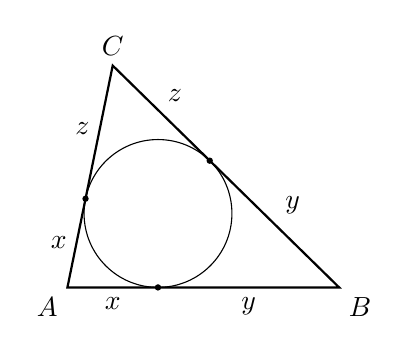
\begin{tikzpicture}[scale=1.15]
  % Triangle de tangentes x = 1, y = 2, z = 1,5 : a = 3,5 ; b = 2,5 ; c = 3.
  \coordinate (A) at (0,0);
  \coordinate (B) at (3,0);
  \coordinate (C) at (0.5,2.4495);
  \coordinate (I) at (1,0.8165);
  \draw[thick] (A) -- (B) -- (C) -- cycle;
  \draw (I) circle (0.8165);
  \fill (1,0) circle (1pt) (0.2,0.9798) circle (1pt) (1.5714,1.3996) circle (1pt);
  \node[below left] at (A) {$A$};
  \node[below right] at (B) {$B$};
  \node[above] at (C) {$C$};
  \node[below] at (0.5,0) {$x$};
  \node[below] at (2,0) {$y$};
  \node[left] at (0.1,0.5) {$x$};
  \node[left] at (0.35,1.75) {$z$};
  \node[above right] at (2.3,0.7) {$y$};
  \node[above right] at (1.0,1.95) {$z$};
\end{tikzpicture}
\end{center}

\subsection*{Le théorème de la bissectrice}

\begin{proposition}\label{prop:bissectrice}
Dans un triangle $ABC$, si la bissectrice intérieure issue de $A$ coupe
$[BC]$ en $D$, alors $\dfrac{BD}{DC} = \dfrac{AB}{AC} = \dfrac cb$.
\end{proposition}

\begin{proof}
Les triangles $ABD$ et $ACD$ ont la même hauteur issue de $A$, donc le
rapport de leurs aires vaut $\frac{BD}{DC}$. Par ailleurs, avec
$\widehat{BAD} = \widehat{DAC} = \frac\alpha2$,
\[
\frac{\mathcal{S}_{ABD}}{\mathcal{S}_{ACD}}
= \frac{\frac12\,AB \cdot AD \sin\frac\alpha2}{\frac12\,AC \cdot AD \sin\frac\alpha2}
= \frac{c}{b} . \qedhere
\]
\end{proof}

\exercice{recueil-8-e1-bissectrices}{Bissectrices et centre du cercle inscrit}

\exercice{recueil-8-e2-weitzenbock}{Inégalité de Weitzenböck}

% ------------------------------------------------------------
\section{À retenir}\label{sec:retenir}

\begin{retenir}
\begin{itemize}
  \item Ramener l'inégalité à une somme de carrés positive.
  \item Inégalités des moyennes, pour des nombres strictement positifs :
  $\min \leqslant H \leqslant G \leqslant A \leqslant Q \leqslant \max$,
  avec égalité si et seulement si tous les nombres sont égaux.
  \item Cauchy--Schwarz, pour des réels quelconques :
  $\left(\sum a_i b_i\right)^2 \leqslant \sum a_i^2 \sum b_i^2$,
  avec égalité si et seulement si les vecteurs sont colinéaires.
  \item Réordonnement : $\sum a_i b_{\sigma(i)}$ est maximale pour deux
  suites rangées dans le même ordre, minimale en ordre inverse.
  \item Dans un triangle, utiliser l'inégalité triangulaire, souvent sous la
  forme $a = y + z$, $b = z + x$, $c = x + y$.
  \item Chercher d'abord le cas d'égalité (souvent : toutes les variables
  égales, ou le triangle équilatéral) : il guide la démonstration.
\end{itemize}
\end{retenir}

% ------------------------------------------------------------
\section{Problèmes}\label{sec:problemes}

\probleme{recueil-8-01-somme-des-produits}{Encadrer $ab + bc + ca$}
\probleme{recueil-8-02-moyenne-ponderee}{Une moyenne pondérée}
\probleme{recueil-8-03-cotes-triangle}{Carrés des côtés d'un triangle}
\probleme{recueil-8-04-oim-1974}{Les valeurs d'une somme de quotients}
\probleme{recueil-8-05-produit-telescopique}{Un produit télescopique}
\probleme{recueil-8-06-serie-telescopique}{Encadrer la somme des inverses des carrés}
\probleme{recueil-8-07-triangle-rectangle}{Puissances des côtés d'un triangle rectangle}
\probleme{recueil-8-08-forme-lineaire-sphere}{Extremums d'une forme linéaire sur la sphère}
\probleme{recueil-8-09-contrainte-xyz}{Sous la contrainte $x^2 + y^2 + z^2 + 2xyz = 1$}

% ------------------------------------------------------------
\ifsolutions
\clearpage
\section{Solutions}\label{sec:solutions}

\solutionde{recueil-8-e1-bissectrices}{Bissectrices et centre du cercle inscrit}{exo}
\solutionde{recueil-8-e2-weitzenbock}{Inégalité de Weitzenböck}{exo}
\solutionde{recueil-8-01-somme-des-produits}{Encadrer $ab + bc + ca$}{pb}
\solutionde{recueil-8-02-moyenne-ponderee}{Une moyenne pondérée}{pb}
\solutionde{recueil-8-03-cotes-triangle}{Carrés des côtés d'un triangle}{pb}
\solutionde{recueil-8-04-oim-1974}{Les valeurs d'une somme de quotients}{pb}
\solutionde{recueil-8-05-produit-telescopique}{Un produit télescopique}{pb}
\solutionde{recueil-8-06-serie-telescopique}{Encadrer la somme des inverses des carrés}{pb}
\solutionde{recueil-8-07-triangle-rectangle}{Puissances des côtés d'un triangle rectangle}{pb}
\solutionde{recueil-8-08-forme-lineaire-sphere}{Extremums d'une forme linéaire sur la sphère}{pb}
\solutionde{recueil-8-09-contrainte-xyz}{Sous la contrainte $x^2 + y^2 + z^2 + 2xyz = 1$}{pb}
\fi

\end{document}
